%-*- mode: LaTeX; -*-

%Consists of Si and C atoms, crystal. (Arranged periodically)
%There exists many (Citation?) different kinds of polytypes
%Polytypes can be thought of as stacking sequence of hexagonal layers
%Base is one C and one Si
%Si and C faces, what is that? [Do I need this?]
%If I do anything on bulk, then I should discuss planes here. (Since the goal is to have (100) plane).

%The atoms are bonded together by covalent bonds.
%The band structure is shown...
%Indirect band gap of...
%Phonons

%Some relevant properties
%Mobility
%Dielectric constant

%Nitrogen as background doping
%Possible acceptors are
%Boron doping gives good band diagram as seen...


\chapter{An introduction to silicon carbide}
\label{sec:sic}
This chapter describes the properties of SiC which are relevant to this thesis. Section \ref{sec:crystal_structure} describes the atomic arrangement in the material, and some different arrangements are discussed. Section \ref{sec:band_structure} discusses the energy band structure of 3C-SiC. Finally section \ref{sec:doping_in_3C} describes how doping is achieved in a material and some of its effects in 3C-SiC. 

\section{Crystal structure}
\label{sec:crystal_structure}
Silicon carbide is a crystalline material consisting of silicon and carbon atoms. The crystalline nature of the material means that the atoms are arranged in a periodically repeating structure called a \emph{lattice}. For given chemical elements there may be several different ways to arrange the atoms in a lattice, i.e. different chemical compounds of the same atomic species. This is called \emph{polytypism}, where the different lattice structures are called the \emph{polytypes} of the material. Silicon carbide has a large number of different polytypes - there are more than 250 known polytypes of SiC \cite{Cheung2006}. The different polytypes can be described as different stacking orders of layers of atoms \cite{Mirgorodsky1995}. Figure \ref{fig:hex} shows one such layer. The depicted layer is the (111) surface. Each circle symbolizes one carbon and one silicon atom, displaced a small distance from each other. This pair of atoms is called the \emph{base} of the crystal. 

\begin{figure}[h]
\begin{center}
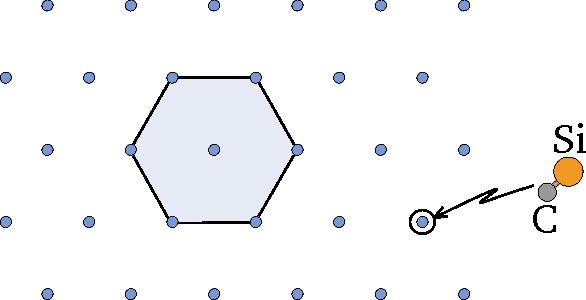
\includegraphics[scale=1]{lattice2.pdf}
\caption{Atomic arrangement of the atoms in each (111) layer. Here each sphere corresponds to one carbon and one silicon atom, as shown by the arrow. 
\label{fig:hex}}
\end{center}
\end{figure}

The marked hexagon in figure \ref{fig:hex} marks an area of the crystal plane which can be used to define the different polytypes, where the polytypes are defined by the placement of the base atoms in this area in different layers. Figure \ref{fig:poly} shows these stacking sequences for three of the most common polytypes. The depicted orders of the layers refer to one period in the periodic structure. The names for the different polytypes are stated at the top of the figure. The digit in the name refers to the number of layers of a period and the letter denotes the crystal symmetry. The letter \emph{H} denotes the hexagonal polytypes, whereas \emph{C} stands for the cubic polytype. Another common polytype is the 6H-SiC, which thus is a hexagonal structure with a period of six base layers. It should be noted that the 2H-SiC structure is the wurtzite structure and the 3C-SiC is the zincblende structure. The unit cell of the zincblende, or 3C-SiC, crystal has a lattice constant of $\mathrm{a} = 4.35$ Å \cite{Bimberg1981}. 


%\begin{figure}[h]
%\begin{center}
%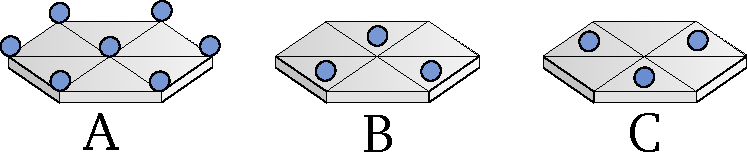
\includegraphics[scale=0.7]{hex5.pdf}
%\caption{Different atomic placements for the layers
%\label{fig:stacking1}}
%\end{center}
%\end{figure}


\begin{figure}[h]
\begin{center}
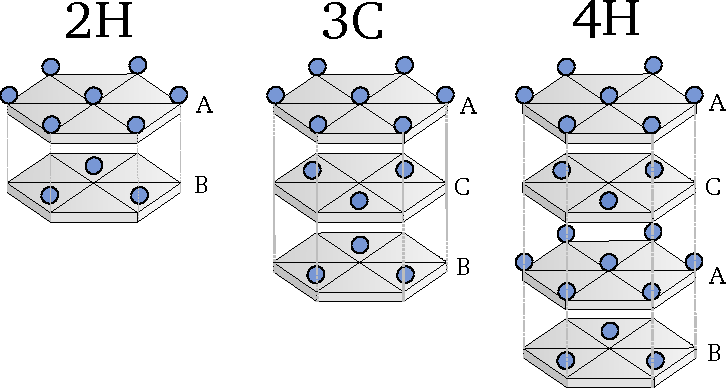
\includegraphics[scale=0.8]{poly.pdf}
\caption{Stacking order for the three most simple polytypes. 
\label{fig:poly}}
\end{center}
\end{figure}

\section{Band structure}
\label{sec:band_structure}
%The atoms are bonded together by covalent bonds.
%The band structure is shown...
%Energy gap - no available energy states
%valence and conduction bands
% Indirect band gap value
	%Change of k, momentum
%Direct band gap value. 

In SiC the atoms are bonded together with covalent bonds into a crystal. When the atoms are bonded together, the energy levels for the electrons in the material are defined by the material and lattice structure. This means that all materials have characteristic energy levels. When many atoms are bound together in a periodically repeating manner, as is the case in crystals, the discrete energy levels for the electrons in the atoms merge together to form continuous bands which are called energy bands. 

The band structure for 3C-SiC is shown as a band diagram in figure \ref{fig:band}. In this figure, each curve describes allowed energies for the electrons, and the spaces in between the curves are not allowed. The x-axis shows different points in reciprocal space, or \emph{k-space}. The marked points are specific points in the first brillouin zone of k-space, and the intermediate intervals form straight lines between the points. This figure has been obtained using the approximate method of pseudopotentials, as described in \cite{Aourag1994}. The zero point energy has been chosen to be at the $\Gamma$-point in k-space. 

The grayed area in the figure is the \emph{band gap} of the material, since there are no allowed electronic states in this area. The band below the band gap is called the valence band, and the band above is called the conduction band. For 3C-SiC, as is characteristic for semiconductors, the Fermi level is in the middle of the band gap. This means that at the temperature of 0 K all electrons will be in the valence band, and the conduction band will be unoccupied. When the conduction band is unoccupied the material will not be able to conduct electricity. If the temperature is raised above 0 K there will be some occupation of the conduction band and some electrical conduction will be possible. With a higher temperature there will be more electrons in the conduction band and thus a higher conductivity of the material. One way to change the position of the Fermi level is to introduce impurities into the crystal, i.e. doping. This will be discussed later. 

\begin{figure}[h]
\begin{center}
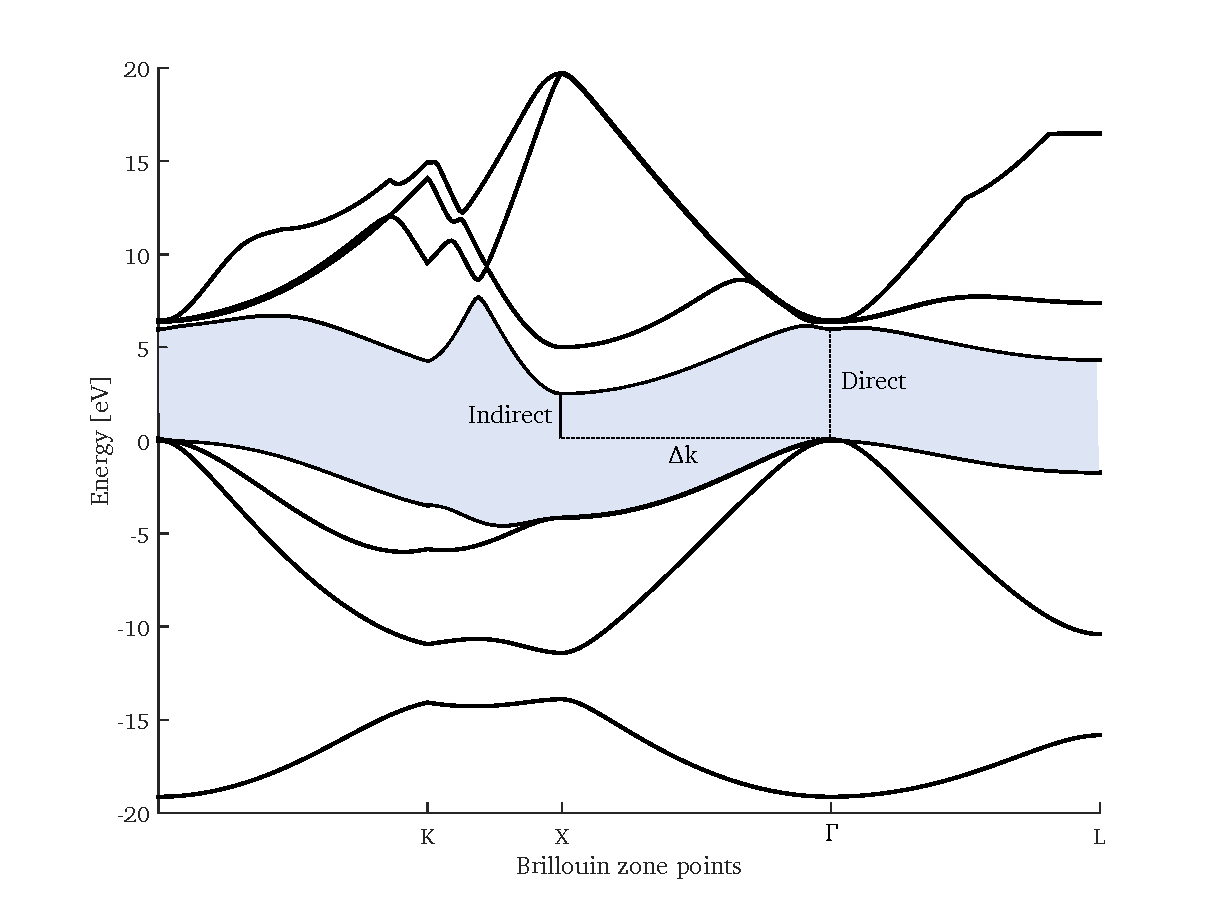
\includegraphics[scale=0.6]{band_diagram2.pdf}
\caption{The band diagram of SiC at ambient conditions for different positions in the Brillouin zone. The indirect and direct band gaps are marked in the figure. The marked area is the band gap. The energy levels have been obtained using the pseudopotential method, as described in \cite{Aourag1994}.
\label{fig:band}}
\end{center}
\end{figure}

In the figure \ref{fig:band} it can be seen that the smallest energy difference between the valence and conduction bands is between the $\Gamma$-point in the valence band and the X-point in the conduction band. This difference is called the \emph{band gap energy}. The difference between the $\Gamma$- and X-points is called the indirect band gap, while the difference between the values at the $\Gamma$-point is called the direct band gap, as illustrated in the figure. These values are given in table \ref{tab:eg}. The value for the room temperature band gaps are taken from the simulation, whereas the 2 K value is taken from literature. 

\begin{table}[h]
\caption{Values for the indirect and direct band gap energies. The indirect values are given both for room temperature and low temperature, as this will be of value later in the thesis.}
\label{tab:eg}
\begin{center}
\begin{tabular}{ l c r }
  \hline                       
  \hline       
  \vspace{1mm}
    $\mathrm{E_{g,indirect}}$  (300 K) & $\mathrm{E_{g,indirect}}$ (2 K) & $\mathrm{E_{g,direct}}$  (300 K)\\
    \hline
  2.36 eV & 2.42 eV \cite{Bimberg1981} & 6.00 eV\\
  \hline  
\end{tabular}
\end{center}
\end{table}

When an electron makes the indirect transition from the valence to the conduction band the energy is increased by E$_\mathrm{g,indirect}$, and the k-value is changed, as indicated by $\Delta \mathrm{k}$ in figure \ref{fig:band}. This change of k-value implies a change in momentum of the electron, since k and momentum p is related by
\[p = \hbar k,\]
where $\hbar$ is Dirac's constant. This is of importance when studying interaction between the material and light. Photons are capable of providing the energy needed to transit from the valence to the conduction band, but cannot provide the change of momentum needed. The law of conservation of momentum requires the total momentum of the system to be preserved during the transitions. The extra momentum can come from interaction with \emph{phonons}, which are vibrations in the crytsal. 

The phonon energy spectrum has four ground modes since there are two different kinds of atoms in the material. There are the acoustic and optical phonon modes. Theoretical calculations of the phonon dispersion curves for 3C-SiC have been done by Karch et al. \cite{Karch1994}. They show the four modes: TA, LA, TO, LO, and give the wavelength for each mode. The transition in k-space for the indirect transition is between the $\Gamma$- and the X-points, hence it is of interest to know which phonon wavelengths and energies this corresponds to.  Table \ref{tab:phonons} shows these computed wavelengths and the corresponding energies, which have been calculated using the fact that

\[E_\mathrm{meV} = \frac{hc(\frac{1}{\lambda_{\mathrm{cm}}})}{e}\times 10^5,\]

\noindent where h is Planck's constant, c is the speed of light and e is the elementary charge. 

\begin{table}[h]
\caption{Inverted wavelengths and energies for the $\Gamma$-X tranistion. Values for $\lambda$ from \cite{Karch1994}.}
\label{tab:phonons}
\begin{center}
\begin{tabular}{ l l l }
  \hline                       
  \hline       
  \vspace{1mm}
    Mode  & $\lambda^{-1} [\mathrm{cm}^{-1}]$  & E [meV]\\
    \hline
  TA &  368 & 45.6\\
  LA &  637 & 79.0\\
  TO &  760 & 94.3\\
  LO &  829 & 102.9\\
  \hline  
\end{tabular}
\end{center}
\end{table}





%\section{Some properties}
%\label{sec:}




\section{Doping in 3C-SiC}
\label{sec:doping_in_3C}

% Doping is when an atom is replaced
% Donors and acceptors, number of valence electrons. 
% Donors can donate, acceptors accept, as seen in fig. 
	% Nitrogen doping, more electrons
	% Ionization energy 
	% Difficult to avoid
	
	% Some possible acceptors
	% And their energies
	% Refer to section about B-doped solar cells. 
% Doping can be achieved...
% Problems which can occur with doping are...


Doping is a way to change the electronic structure of a material by substituting some of the native atoms with a foreign element. In the case of SiC this means that either silicon or carbon is replaced by some other element. The band structure of the material changes depending on which impurity is introduced to the crystal. By choosing the dopants it is possible to tailor the band structure to create various new properties of the material. 

An important factor for how the band structure is changed is the number of valence electrons in the introduced element, compared to the element it replaces. Silicon and carbon both have four valence electrons, creating four bonds to its neighbouring atoms in the crystal. The electrons are strongly bound to the atomic nuclei, requiring energy corresponding to the band gap to free one electron. If one silicon or one carbon atom is replaced by an element with five valence electrons, the additional electron is not as strongly bound to the nucleus and can easily release an electron to the conduction band. This is called a \emph{donor} atom. Similarly if an atom with only three valence electrons is introduced to the crystal, it can readily bind an electron from the valence band, creating an electron deficiency, or \emph{hole} in the valence band. This is called an \emph{acceptor} atom. Figure \ref{fig:dopant_band} shows a simplified band diagram with a donor and an acceptor level. The donor level donates an electron to the conduction band when the electron is supplied with the energy $\mathrm{E_D}$. The acceptor accepts an electron from the valence band when the electron is supplied with the energy $\mathrm{E_A}$. The energy required to supply the material with one carrier from a dopant level is called the \emph{binding energy} (or \emph{ionization energy}) of the dopant. 

\begin{figure}[h]
\begin{center}
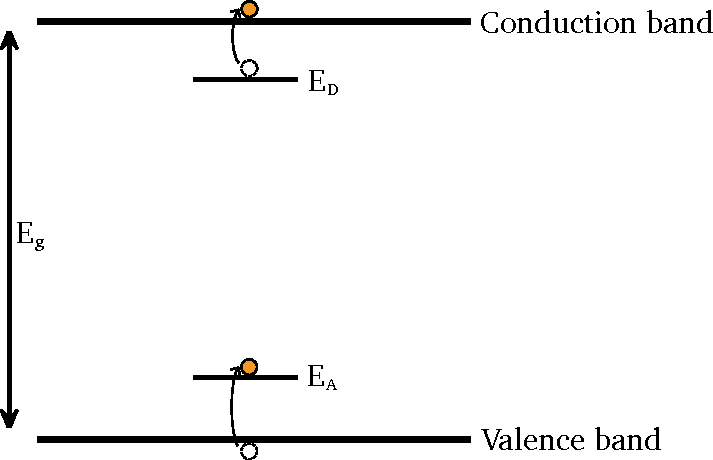
\includegraphics[scale=0.6]{doped_band1.pdf}
\caption{Two new energy levels are introduced by doping. 
\label{fig:dopant_band}}
\end{center}
\end{figure}

As dopants are introduced in the material, the position of the Fermi level relative to the bands changes. The Fermi level resides in the middle of the band for undoped materials, but will move nearer to the conduction (valence) band as donors (acceptors) are introduced. This change in Fermi energy corresponds to a change in occupancy in the different levels. 

\subsection{Donors}
% What does it replace, Si or C?
Since silicon and carbon both have four valence electrons, a donor atom in SiC must have five or more electrons. One common donor is nitrogen, which has five valence electrons. The nitrogen atoms take the place of the carbon atoms in the lattice. This means that each added N-atom can supply the conduction band with one electron. A material with more electron carriers than the hole counterpart is said to be an \emph{n-type} material. Freitas et al. have measured the binding energy of nitrogen in 3C-SiC, and found it to be 54 meV \cite{Freitas1988}. This means that the lowest N-level is 54 meV below the conduction band.

Nitrogen doping can be achieved intentionally by fabricating the material in a nitrogen atmosphere, but nitrogen is always present in sublimation grown material even at vacuum conditions \cite{Sun2012b}. This means that material grown by this method is generally n-type, if no other impurity is present. The n-type material can also be created by other elements in group five.  Another possible donor in 3C-SiC is phosphorus, which has a binding energy of 48 meV \cite{Ivanov2010}. Reports of doping with As, P and Sb exist, but are far less common than N-doping \cite{Rao1999}. 

\subsection{Acceptors}
% What do they replace, Si or C?
Acceptor atoms need to have fewer valence electrons than silicon and carbon, which is why group three elements are the most common acceptors. Examples of acceptor materials are boron and aluminium, which have the binding energies 257 meV \cite{Freitas1988} and 735 meV \cite{Richards2003} respectively. A material with more hole carriers than the electron counterpart is said to be \emph{p-type}. Table \ref{tab:dopants} summarizes the different dopant energy levels. 

\begin{table}[h]
\caption{Binding energies for some of the most common SiC dopants.}
\label{tab:dopants}
\begin{center}
\begin{tabular}{ l l l r}
  \hline                       
  \hline       
  \vspace{1mm}
    Element  & Dopant type & E$_{D/A}$ [meV] & Reference\\
    \hline
  N &  Donor & 54 & \cite{Freitas1988}\\
  B &  Acceptor & 735 & \cite{Richards2003}\\
  Al &  Acceptor & 257  & \cite{Freitas1988}\\
  \hline  
\end{tabular}
\end{center}
\end{table}

The B-doping energy level is of particular interest for photovoltaic applications, where the binding energy is ideal for an application called \emph{intermediate band photovoltaic solar cell}. In this application, the electrons can make two different energy transitions. One transition can be done between the valence band and the impurity level, and one between the impurity  level and the conduction band. It has been shown that the binding energy of the B-acceptor in 3C-SiC is very well matched to the solar spectrum. Much of the emitted solar energy can be captured by the B-doped 3C-SiC \cite{Richards2003,Luque1997}. 
%This is described in more detail in chapter \ref{sec:intermediate_band_pvc}. 
\\ 

\noindent 
There are several ways to create doped materials. It can be done by ion implantation, where ions are accelerated to high energies and then made to collide with the undoped material \cite{Rao1999}. It can also be done as the material is grown, by including the doping element in the ambient. The first method has several advantages: it can be done with good control over doping density and it is possible to select only certain areas of the material to dope. The latter method is done \emph{in situ}, so it requires no additional equipment. It is also not as prone to create defects as the ion implantation method is, where annealing is often required after implantation in order to reduce the number of defects. In the work described in this thesis, the method of doping is to include the doping material during the growth. This method is described in more detail in chapter \ref{sec:growth}. 

During doping some of the native atoms are replaced. This will have effects on the quality of the produced material. Different elements have different atomic radii, so replacing one atom by one of a different element will create some strain in the material. This may lead to defects in the material. 




































